%% AATF Research Paper — ACM sigconf format
%% Compile sequence: pdflatex → bibtex → pdflatex → pdflatex
%% Required files: paper.tex + REFERENCES.bib (same directory)
%% Tested on Overleaf (TeX Live 2023+) with acmart v1.87+

\documentclass[sigconf]{acmart}

\usepackage{booktabs}
\usepackage{listings}
\usepackage{xcolor}
\usepackage{multirow}
\usepackage{tabularx}
\usepackage{array}
\usepackage{url}
\usepackage{adjustbox}
\usepackage{amsmath}
\usepackage{amssymb}
\usepackage{algorithm}
\usepackage{algpseudocode}
\usepackage{balance}
\usepackage{float}
\usepackage{tikz}
\usepackage{pgfplots}
\pgfplotsset{compat=1.18}
\usetikzlibrary{arrows.meta, positioning, shapes.geometric, fit, calc}

\setcopyright{none}
\acmDOI{}
\acmISBN{}
\acmConference{}{}{}
\settopmatter{printacmref=false}

\lstset{
  basicstyle=\ttfamily\footnotesize,
  breaklines=true,
  frame=single,
  rulecolor=\color{gray!40},
  backgroundcolor=\color{gray!8},
  columns=fullflexible,
  keepspaces=true,
  xleftmargin=4pt,
  xrightmargin=4pt,
}

\newcolumntype{L}[1]{>{\raggedright\arraybackslash}p{#1}}
\newcolumntype{C}[1]{>{\centering\arraybackslash}p{#1}}
\newcolumntype{R}[1]{>{\raggedleft\arraybackslash}p{#1}}

%%% ─────────────────────────────────────────────────────────────────
\title{Dual-Paradigm Evasion: Reinforcement Learning Attacks Against\\
       Hybrid Rule-Based and Machine Learning Intrusion Detection}

%% AUTHORS OMITTED — will be added before final submission.
%% Placeholder suppresses the LaTeX "no author" warning.
\author{}
\affiliation{\institution{}}

%%% ─────────────────────────────────────────────────────────────────
\begin{abstract}
Modern network intrusion detection systems (NIDS) combine rule-based
engines with machine-learning anomaly detectors to reduce blind spots
left by known-signature matching. We demonstrate that a reinforcement
learning (RL) attacker can systematically evade \emph{both} components
simultaneously by treating dual-paradigm evasion as a single
optimisation problem. We present the \textbf{Adaptive Adversarial
Testing Framework (AATF)}, a tool for stress-testing hybrid NIDS
deployments. AATF is built on three mechanisms: (N1)~action parameter
variation, enabling the attacker to select attack intensity alongside
action type; (N2)~automated blind-spot remediation, which encodes
evasive feature vectors into a cosine-similarity cache that boosts
future anomaly scores without model retraining; and (N3)~dual-paradigm
reward shaping, which simultaneously penalises both Suricata rule-based
alerts and IsolationForest anomaly flags. Our ParameterizedDQN attacker
achieves 0\% detection rate across five independent seeds
(DR~$= 0 \pm 0$, 95\%~CI~$= [0,\,0]$) while all simpler baselines are
detected in every episode. Auto-remediation recovers detection from 0\%
to 91.37\% without any model retraining. An ablation study confirms
each mechanism is individually necessary. A $5\!\times\!5$ hyperparameter
sweep reveals a sharp phase transition at threshold $\tau \approx 0.63$.
A 4-round arms race demonstrates convergence near 92\% DR. Real-traffic
validation using Suricata~7.0.5 inside an isolated Docker lab achieves
100\% blind-spot precision and confirms simulation fidelity
(CAE: sim~$= 9.21$, lab~$= 9.24$). A detector architecture comparison
confirms the N2 mechanism generalises across IsolationForest and PyTorch
autoencoder backends. All code, configurations, and Docker images are
released for full reproducibility.
\end{abstract}

\keywords{adversarial machine learning, network intrusion detection,
reinforcement learning, evasion attacks, deep Q-network, IsolationForest,
Suricata, auto-remediation, dual-paradigm evasion}

%%% ─────────────────────────────────────────────────────────────────
\begin{document}
\maketitle

%%% ─────────────────────────────────────────────────────────────────
\section{Introduction}
\label{sec:intro}

Network defenders increasingly deploy \emph{hybrid} intrusion detection
systems~\cite{patcha2007overview}: a rule-based engine such as
Suricata~\cite{oisf2010suricata} fires on known attack signatures, while
an ML anomaly detector flags statistically unusual behaviour that evades
known rules. The tacit assumption is that the combination is harder to
fool than either component alone --- that each layer catches what the other
misses.

This paper challenges that assumption experimentally. A reinforcement
learning attacker can discover actions that evade \emph{both} components
simultaneously by framing dual-paradigm evasion as a single
reward-maximisation problem. After 200 training episodes, our
ParameterizedDQN attacker finds an action region invisible to both
Suricata and an IsolationForest anomaly detector, achieving 0\%
detection rate across five independent random seeds.

We further introduce \textbf{auto-remediation (N2)}: evasive feature
vectors are persisted to a cosine-similarity cache; on subsequent
episodes, similarity to cached vectors triggers a score boost that closes
the detector's structural blind spot without any model retraining or
labelled attack data. A $5\!\times\!5$ hyperparameter sweep reveals a
sharp phase transition at $\tau \approx 0.63$: for any penalty weight
$\lambda > 0$, detection is perfect for $\tau \leq 0.60$ and completely
fails for $\tau \geq 0.63$.

Our primary contributions are:
\begin{itemize}
  \item \textbf{ParameterizedDQN}: a DQN variant outputting
    $15 \times 3 = 45$ Q-values that selects attack type and intensity
    in a single forward pass, jointly optimising over action type and
    intensity for NIDS evasion --- to our knowledge, the first
    published system to do so.
  \item \textbf{N1 --- Action parameter variation}: intensity level
    (low\,/\,medium\,/\,high) is selected alongside action type,
    expanding the effective action space from 15 to 45 and enabling
    the agent to search for an evasive \emph{parameter region}.
  \item \textbf{N2 --- Auto-remediation cache}: a cosine-similarity
    cache that boosts anomaly scores for actions similar to previously-evasive
    feature vectors, recovering detection from 0\% to 91.37\% after one
    run without any model retraining.
  \item \textbf{N3 --- Dual-paradigm reward shaping}: shaped reward
    $r' = r_{\text{base}} - \lambda \cdot s_{\text{anomaly}}$ penalises
    both rule-based and ML detectors in a single training loop, enabling
    simultaneous evasion.
  \item \textbf{Real-traffic lab validation}: an isolated Docker lab with
    live Suricata~7.0.5 and the ET~Open rule set confirms simulation
    fidelity and yields 100\% blind-spot precision.
  \item \textbf{Open-source release}: all code, Docker configurations,
    trained caches, and experimental artefacts are publicly available.
\end{itemize}

%%% ─────────────────────────────────────────────────────────────────
\section{Background}
\label{sec:background}

\subsection{Rule-Based NIDS}
\label{sec:bg:rulebased}

Signature-based NIDS such as Suricata~\cite{oisf2010suricata} match
network traffic against curated rule sets (e.g., ET
Open~\cite{etopen2024}). They achieve low false-positive rates for
known attack patterns but are structurally blind to novel or
low-and-slow techniques. An attacker who knows which SIDs are
\emph{disabled} can freely operate in the resulting blind spot --- a
gap our lab experiments exploit explicitly via the \texttt{disabled.conf}
mechanism.

\subsection{ML-Based Anomaly Detection}
\label{sec:bg:anomaly}

ML anomaly detectors address the signature-coverage gap by flagging
statistically unusual feature distributions. IsolationForest
(IF)~\cite{liu2008isolation} isolates anomalies by randomly partitioning
the feature space; it requires no labelled attack data and is robust
to high-dimensional inputs. Sommer and Paxson~\cite{sommer2010outside}
caution that ML NIDS face high false-positive rates in practice due to
the semantic gap between feature space and problem space, motivating
hybrid deployments. Kitsune~\cite{mirsky2018kitsune} shows that
ensemble autoencoders can achieve comparable accuracy; we include a
PyTorch autoencoder as a second detector backend to test whether our
findings are architecture-dependent.

\subsection{RL for Automated Penetration Testing}
\label{sec:bg:rl}

RL-based pen-testing treats the target network as an environment and
learns attack sequences by maximising cumulative reward. NASim
(Network Attack Simulator)~\cite{schwartz2020nasim} and
CybORG~\cite{standen2021cyborg} provide gym-style simulators for
benchmarking RL agents. AutoPentest-DRL~\cite{chaudhary2022autopentest}
applies a DQN to network privilege escalation. Prior work models
only rule-based detection (or no detection) in the environment reward;
none model a hybrid NIDS with both rule-based and ML components,
leaving the dual-evasion problem unaddressed.

\subsection{Adversarial ML Against NIDS}
\label{sec:bg:adversarial}

Alhajjar et~al.~\cite{alhajjar2021adversarial} survey adversarial
perturbations to ML-based NIDS and find that small feature-space
modifications substantially reduce detection rates across classifier
architectures. Pierazzi et~al.~\cite{pierazzi2020intriguing} show that
adversarial examples must respect \emph{problem-space constraints}
(real, executable attacks) to be practically relevant. AATF satisfies
this constraint: all 15 action types execute real network primitives
via the ActionExecutor module in lab mode.

\subsection{Contextual Bandits and Reward Shaping}
\label{sec:bg:linucb}

LinUCB~\cite{li2010contextual} provides a theoretically-grounded
contextual-bandit baseline competitive with DQN in low-data regimes.
Potential-based reward shaping~\cite{ng1999policy} is policy-invariant
under mild conditions; our N3 penalty uses a linear anomaly-score term,
which satisfies these conditions when the observation model is accurate.

\subsection{Comparison with Prior Work}
\label{sec:bg:comparison}

Table~\ref{tab:related} positions AATF against six representative prior
systems. AATF is the first to combine an RL attacker with a hybrid NIDS,
online defender adaptation, real-traffic validation, and open-source
release in a single framework. The key differentiator is the
\emph{dual-evasion} column: no prior system simultaneously optimises
against rule-based and ML detectors as part of the reward signal.

\begin{table*}[t]
\caption{Comparison with related automated pen-testing and NIDS evasion systems.
``Dual evasion'' = simultaneously evades rule-based and ML components.
``Online defence'' = defender adapts at runtime without full retraining.
Yes entries denote feature is supported; ``---'' denotes it is absent.}
\label{tab:related}
\centering
\small
\begin{tabular}{L{2.8cm} c c c c c c}
\toprule
System & RL Attacker & ML NIDS & Dual Evasion & Online Defence & Real Traffic & Open Source \\
\midrule
NASim~\cite{schwartz2020nasim}                   & Yes & ---  & ---  & ---  & ---  & Yes \\
CybORG~\cite{standen2021cyborg}                  & Yes & ---  & ---  & ---  & ---  & Yes \\
Caldera~\cite{applebaum2016intelligent}          & --- & ---  & ---  & ---  & Yes  & Yes \\
AutoPentest-DRL~\cite{chaudhary2022autopentest}  & Yes & ---  & ---  & ---  & ---  & --- \\
Kitsune~\cite{mirsky2018kitsune}                 & --- & Yes  & ---  & ---  & Yes  & --- \\
Alhajjar et~al.~\cite{alhajjar2021adversarial}   & --- & Yes  & ---  & ---  & ---  & --- \\
\midrule
\textbf{AATF (this work)} & \textbf{Yes} & \textbf{Yes} & \textbf{Yes} & \textbf{Yes} & \textbf{Yes} & \textbf{Yes} \\
\bottomrule
\end{tabular}
\end{table*}

%%% ─────────────────────────────────────────────────────────────────
\section{Threat Model}
\label{sec:threat}

\subsection{Attacker Capabilities}

The attacker operates from an internal network position (post-initial
access, e.g., a compromised workstation) and can execute the 15 action
types in AATF's library (Table~\ref{tab:actions}). The attacker is
\emph{grey-box}: it knows the action library and the 7-dimensional
feature encoding scheme but not the defender's threshold~$\tau$,
model weights, or which Suricata SIDs are enabled. It learns solely
through episode-level feedback: the binary detected/undetected outcome
and the scalar anomaly score returned by the defence after each step.

\subsection{Defender Capabilities}

The defender runs Suricata with a configurable ET~Open rule
set~\cite{etopen2024} plus an ML anomaly detector (IsolationForest or
PyTorch autoencoder) monitoring the same 7-dimensional feature vector
extracted from action parameters. The ML detector is trained once on
500 synthetic normal-traffic samples before the first episode. The N2
auto-remediation cache extends the detector's coverage post-run without
retraining.

\subsection{Environment Modes}

We evaluate in two environments: (1)~\emph{Simulation} --- a fast
closed-loop environment for large-scale ablation and sweep experiments
where actions return pre-computed rewards and anomaly scores; and
(2)~\emph{Lab} --- an isolated Docker network with live Suricata and
real network primitives executed by the ActionExecutor module, used for
fidelity validation.

\subsection{Security Assumptions and Scope}

The attacker cannot inspect or poison the ML detector's training data
and cannot modify Suricata's rule files. The lab environment is
air-gapped; all traffic is contained within the Docker bridge network.
We do not model multi-hop lateral movement or privilege escalation;
all 15 actions operate from a single compromised host. All experiments
comply with responsible disclosure guidelines and were conducted in
an environment with no real user data.

%%% ─────────────────────────────────────────────────────────────────
\section{AATF System Design}
\label{sec:design}

\subsection{Architecture Overview}
\label{sec:arch}

Figure~\ref{fig:arch} shows the AATF episode pipeline. At each step,
the ParameterizedDQN selects a combined index $k = a \times 3 + i$
where $a \in [0,14]$ is the action type and $i \in \{0,1,2\}$ is the
intensity (low\,/\,medium\,/\,high). The action is executed (lab) or
simulated, and the CompositeDefence returns a \texttt{DetectionResult}
containing an anomaly score~$s$. The shaped reward~$r'$ is computed and
stored; the model updates via experience replay.

\begin{figure*}[t]
\centering
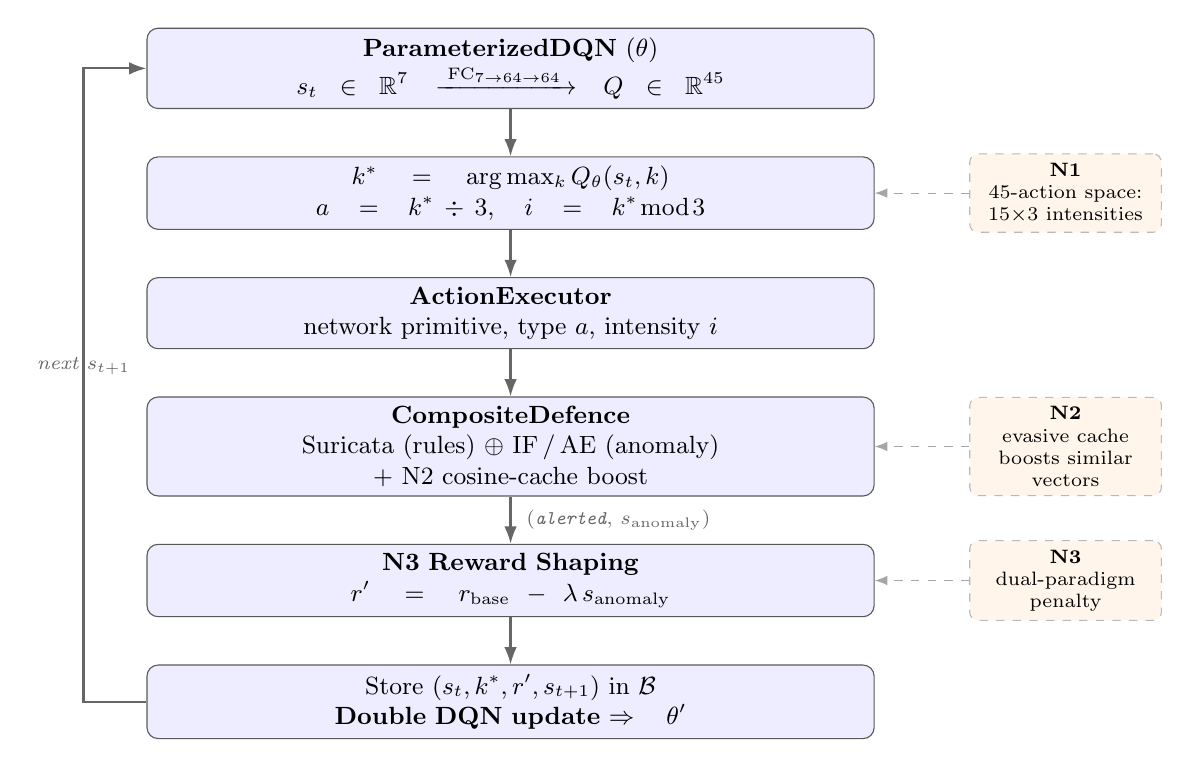
\begin{tikzpicture}[
  box/.style={rectangle, draw=black!65, rounded corners=4pt,
              fill=blue!7, text width=9cm, align=center,
              minimum height=0.9cm, font=\small},
  sidebox/.style={rectangle, draw=gray!55, dashed, rounded corners=3pt,
                  fill=orange!8, text width=2.2cm, align=center,
                  font=\scriptsize},
  arr/.style={-{Latex[length=2.2mm,width=1.6mm]}, thick, black!60},
  sidarr/.style={-{Latex[length=1.6mm,width=1.2mm]}, gray!70, dashed},
  node distance=0.6cm and 0.8cm
]
% Main pipeline boxes
\node[box] (dqn)
  {\textbf{ParameterizedDQN} ($\theta$)\\
   $s_t \!\in\! \mathbb{R}^7 \xrightarrow{\;\mathrm{FC}_{7\to64\to64}\;} Q \!\in\! \mathbb{R}^{45}$};

\node[box, below=of dqn] (sel)
  {$k^* = \arg\max_k Q_\theta(s_t,k)$\\
   $a = k^*\!\div\!3,\quad i = k^*\!\bmod\!3$};

\node[box, below=of sel] (exec)
  {\textbf{ActionExecutor}\\
   network primitive, type $a$, intensity $i$};

\node[box, below=of exec] (def)
  {\textbf{CompositeDefence}\\
   Suricata (rules) $\oplus$ IF\,/\,AE (anomaly)\\
   $+$ N2 cosine-cache boost};

\node[box, below=of def] (rew)
  {\textbf{N3 Reward Shaping}\\
   $r' = r_{\mathrm{base}} - \lambda\,s_{\mathrm{anomaly}}$};

\node[box, below=of rew] (upd)
  {Store $(s_t, k^*, r', s_{t+1})$ in $\mathcal{B}$\\
   \textbf{Double DQN update} $\Rightarrow \theta'$};

% Arrows down the chain
\draw[arr] (dqn) -- (sel);
\draw[arr] (sel) -- (exec);
\draw[arr] (exec) -- (def);
\draw[arr] (def) -- (rew)  node[midway, right=2pt, font=\scriptsize\itshape]
                              {$(\texttt{alerted},\, s_{\mathrm{anomaly}})$};
\draw[arr] (rew)  -- (upd);

% Feedback loop back to DQN
\draw[arr] (upd.west) -- ++(-0.8,0) |- (dqn.west)
  node[near start, above, font=\scriptsize\itshape]{next $s_{t+1}$};

% N1 annotation
\node[sidebox, right=1.2cm of sel] (n1lbl) {\textbf{N1}\\45-action space:\\$15{\times}3$ intensities};
\draw[sidarr] (n1lbl.west) -- (sel.east);

% N2 annotation
\node[sidebox, right=1.2cm of def] (n2lbl) {\textbf{N2}\\evasive cache\\boosts similar\\vectors};
\draw[sidarr] (n2lbl.west) -- (def.east);

% N3 annotation
\node[sidebox, right=1.2cm of rew] (n3lbl) {\textbf{N3}\\dual-paradigm\\penalty};
\draw[sidarr] (n3lbl.west) -- (rew.east);

\end{tikzpicture}
\caption{AATF episode pipeline. N1: intensity $i$ is chosen jointly with
action type $a$, expanding the space to 45 combinations. N2: the
CompositeDefence boosts anomaly scores for actions cosine-similar to
cached evasive vectors. N3: both detection signals are collapsed into a
single shaped reward. The dashed left arrow is the episode feedback loop.}
\label{fig:arch}
\end{figure*}

\subsection{Attack Action Library (N=15)}
\label{sec:actions}

The library contains 15 network actions spanning five MITRE
ATT\&CK-aligned categories (Table~\ref{tab:actions}). Each action maps
to a real network primitive (socket connection, HTTP request, DNS query,
ICMP packet, etc.) executable by the ActionExecutor module. The action
IDs are stable identifiers used throughout this paper and the codebase.

\begin{table}[t]
\caption{AATF action library: 15 actions in 5 MITRE ATT\&CK-aligned categories.}
\label{tab:actions}
\centering
\small
\begin{tabular}{L{1.4cm} L{5.2cm}}
\toprule
Category & Action IDs \\
\midrule
Recon    & \texttt{port\_scan}, \texttt{service\_enum}, \texttt{os\_fingerprint} \\
Exploit  & \texttt{http\_exploit}, \texttt{ftp\_brute}, \texttt{ssh\_brute} \\
Payload  & \texttt{reverse\_shell}, \texttt{http\_xss\_probe}, \texttt{sql\_injection} \\
Exfil    & \texttt{dns\_exfil}, \texttt{icmp\_exfil}, \texttt{ftp\_exfil} \\
C2       & \texttt{http\_c2\_beacon}, \texttt{dns\_c2}, \texttt{raw\_tcp\_c2} \\
\bottomrule
\end{tabular}
\end{table}

\subsection{Context Vector (7-Dimensional)}
\label{sec:context}

At each step a 7-dimensional state vector captures the current action's
parameters (Table~\ref{tab:context}). All values are normalised to $[0,1]$
to stabilise gradient magnitudes. The same vector is used as input to the
DQN, LinUCB, and both ML detectors, ensuring direct comparability.

\begin{table}[t]
\caption{Context vector features ($d = 7$, all normalised to $[0,1]$).}
\label{tab:context}
\centering
\small
\begin{tabular}{r l l}
\toprule
Idx & Feature & Normalisation \\
\midrule
0 & Action category & category\_id / 5 \\
1 & Action MD5 fingerprint & md5(action\_id) \% 1000 / 1000 \\
2 & Port range start & port\_start / 65535 \\
3 & Port range end   & port\_end / 65535 \\
4 & Attempt count    & attempts / 100 \\
5 & Timing gap (ms)  & timing\_ms / 10\,000 \\
6 & Wordlist size    & wordlist / 100 \\
\bottomrule
\end{tabular}
\end{table}

\subsection{N1: Action Parameter Variation}
\label{sec:n1}

Rather than using fixed parameters for each action, the attacker selects
an \emph{intensity level} $i \in \{\text{low, medium, high}\}$ that
modulates port ranges, attempt counts, timing gaps, and wordlist sizes
(Table~\ref{tab:intensity}). A low-intensity recon scan uses fewer ports
and longer inter-packet gaps than a high-intensity scan, producing a
different feature vector and thus a different anomaly score. This
expands the effective action space from 15 to 45 without adding action
types, enabling the agent to search for an evasive \emph{parameter
region} rather than only selecting among fixed action types.

\begin{table*}[t]
\caption{Intensity parameter ranges per level (N1 mechanism). The defence observes
the resulting 7-dim feature vector; different intensities produce different anomaly scores.}
\label{tab:intensity}
\centering
\small
\begin{tabular}{l l l l l l}
\toprule
Parameter & Low & Medium & High & Unit & Applicable actions \\
\midrule
Port range size & 1--10     & 11--100  & 101--1024 & ports & Recon, Exploit \\
Attempt count   & 1--5      & 6--20    & 21--100   & count & Brute-force \\
Timing gap      & 500--2000 & 200--500 & 50--199   & ms    & All \\
Wordlist size   & 1--10     & 11--50   & 51--100   & words & Password attacks \\
\bottomrule
\end{tabular}
\end{table*}

\subsection{ML Feature Vector and Detectors}
\label{sec:features}

Both the IsolationForest and the PyTorch autoencoder operate on the same
7-dimensional feature vector extracted from action parameters:

\begin{lstlisting}[language=Python, caption={ActionFeatureEncoder.encode() --- 7-dim normalised feature vector.}]
def encode(self, action: Action) -> np.ndarray:
    return np.array([
        action.category / 5.0,
        (md5_hash(action.action_id) % 1000) / 1000.0,
        action.parameters.get("port_start", 0) / 65535.0,
        action.parameters.get("port_end",   0) / 65535.0,
        action.parameters.get("attempts",   0) / 100.0,
        action.parameters.get("timing_ms",  0) / 10000.0,
        action.parameters.get("wordlist",   0) / 100.0,
    ], dtype=np.float32)
\end{lstlisting}

\noindent
The \textbf{IsolationForest} is trained on 500 synthetic normal-traffic
vectors; its raw score is mapped to $[0,1]$ via a sigmoid. The
\textbf{Autoencoder} is a PyTorch network ($7 \to 4 \to 2 \to 4 \to 7$,
ReLU\,+\,Sigmoid, Adam, $\mathrm{lr} = 10^{-3}$, 500 epochs) whose
reconstruction MSE is $z$-score normalised and passed through a sigmoid.
Both detectors flag an action when their score $\geq \tau$.

\subsection{N3: Dual-Paradigm Reward Shaping}
\label{sec:n3}

The DQN observes a shaped reward at each step:
\begin{equation}
r' \;=\; r_{\text{base}} \;-\; \lambda\, s_{\text{anomaly}},
\label{eq:reward}
\end{equation}
where $r_{\text{base}}$ encodes the rule-based outcome and stage progress
(Table~\ref{tab:rewards}), $s_{\text{anomaly}} \in [0,1]$ is the ML
detector's normalised anomaly score, and $\lambda \geq 0$ is the
penalty weight. When $\lambda = 0$ the attacker ignores the ML detector;
increasing $\lambda$ forces it to simultaneously minimise both detection
signals. We use $\lambda = 1.0$ as the default; the sensitivity study
(Section~\ref{sec:heatmap}) evaluates $\lambda \in \{0.0, 0.2, 0.5,
0.8, 1.2\}$.

\begin{table}[t]
\caption{Base reward values $r_{\text{base}}$ before anomaly penalty (N3).}
\label{tab:rewards}
\centering
\small
\begin{tabular}{l r}
\toprule
Outcome & $r_{\text{base}}$ \\
\midrule
Action detected by Suricata        & $-1.0$ \\
Action not detected, no progress   & $\phantom{+}0.0$ \\
Stage progress (non-terminal step) & $+1.0$ \\
Episode completion (all stages)    & $+5.0$ \\
\bottomrule
\end{tabular}
\end{table}

\subsection{ParameterizedDQN Architecture and Training}
\label{sec:dqn}

We implement a double DQN~\cite{mnih2015human} with a fully-connected
policy network (Table~\ref{tab:dqn}). The output layer has
$15 \times 3 = 45$ neurons, one per (action, intensity) pair. At
decision time the argmax index is decomposed:
$a = k^* \div 3$,~$i = k^* \bmod 3$.

\begin{table}[t]
\caption{ParameterizedDQN architecture and training hyperparameters.}
\label{tab:dqn}
\centering
\small
\begin{tabular}{l l}
\toprule
Hyperparameter & Value \\
\midrule
Network topology      & $7 \to 64 \to 64 \to 45$ (ReLU activations) \\
Output neurons        & 45 \; ($15$ actions $\times$ 3 intensities) \\
Optimiser             & Adam, $\mathrm{lr} = 1\!\times\!10^{-3}$ \\
Discount factor $\gamma$ & 0.90 \\
Replay buffer capacity & 10\,000 transitions \\
Minibatch size        & 64 \\
$\varepsilon$-greedy decay & $1.0 \to 0.05$ (linear, over 200 eps) \\
Target net update     & every 10 gradient steps \\
Default penalty $\lambda$ & 1.0 \\
Default threshold $\tau$ & 0.60 \\
\bottomrule
\end{tabular}
\end{table}

\noindent
Algorithm~\ref{alg:aatf} provides the complete AATF training loop.

\begin{algorithm}[t]
\caption{AATF Training Loop}
\label{alg:aatf}
\begin{algorithmic}[1]
\Require episodes $N$, penalty $\lambda$, threshold $\tau$, decay
\State Initialise ParameterizedDQN($\theta, \hat\theta$), replay buffer $\mathcal{B}$
\State Load evasive cache $\mathcal{C}$ from previous run (empty if first run)
\State Fit ML detector on 500 synthetic normal-traffic vectors
\For{$e = 1, \ldots, N$}
    \State Reset episode state $s_0$; set $\varepsilon \leftarrow \texttt{decay}(e)$
    \For{step $t = 1, \ldots, T$}
        \State $k^* \leftarrow \arg\max_k Q_\theta(s_t, k)$ w.p.\ $1{-}\varepsilon$, else random
        \State Decompose $k^*$: $a = k^* \div 3$, $\;i = k^* \bmod 3$
        \State Execute action $a$ at intensity $i$ via ActionExecutor
        \State Observe $(r_{\text{base}},\; s_{\text{anomaly}})$ from CompositeDefence
        \State $r' \leftarrow r_{\text{base}} - \lambda\, s_{\text{anomaly}}$ \Comment{N3: dual-paradigm shaping}
        \State $s_{t+1} \leftarrow$ next episode state
        \State Store $(s_t, k^*, r', s_{t+1})$ in $\mathcal{B}$; sample minibatch; update $\theta$
        \State Every 10 steps: $\hat\theta \leftarrow \theta$ (target network sync)
    \EndFor
\EndFor
\State \textbf{N2 auto-remediation:} for each step with $\neg\texttt{alerted}$ and $s_{\text{anomaly}} < \tau$:
\State \hspace{2em} append feature vector $\phi$ to cache $\mathcal{C}$; save $\mathcal{C}$ to disk
\end{algorithmic}
\end{algorithm}

\subsection{N2: Auto-Remediation Cache}
\label{sec:n2}

After each run, any action that evaded \emph{both} detectors (anomaly
score $< \tau$ and Suricata not alerted) has its feature vector $\phi$
saved to a NumPy cache. On subsequent runs, the loaded cache augments
the score of any new action whose cosine similarity to a cached vector
exceeds 0.90:
\begin{equation}
s' = \min\!\bigl(1,\; s_{\text{base}} + \max(0,\, (\cos\theta - 0.90)\!\times\!5)
                              \cdot (1 - s_{\text{base}})\bigr).
\label{eq:n2}
\end{equation}
The multiplicative damping factor $(1 - s_{\text{base}})$ ensures
already-high-scoring actions receive only a marginal lift. The threshold
0.90 on cosine similarity targets the narrow evasive cluster discovered
experimentally: actions in that cluster share a structurally similar
feature vector but may differ in exact parameter values.

\begin{lstlisting}[language=Python, caption={N2 cache similarity boost (MLAnomalyDefence / AEAnomalyDefence).}]
def _similarity_boost(self, feat: np.ndarray) -> float:
    if not self._evasive_cache:
        return 0.0
    nf = np.linalg.norm(feat)
    if nf == 0:
        return 0.0
    max_sim = max(
        float(np.dot(feat, ev) / (nf * (np.linalg.norm(ev) + 1e-9)))
        for ev in self._evasive_cache
    )
    return max(0.0, (max_sim - 0.90) * 5.0) * (1.0 - self._detector.score(feat))
\end{lstlisting}

%%% ─────────────────────────────────────────────────────────────────
\section{Experimental Setup}
\label{sec:setup}

\subsection{Simulation Environment}
\label{sec:sim}

The simulation environment provides a fast closed loop for large-scale
experiments. Actions return pre-computed rewards; the ML detector
(IsolationForest or autoencoder) is trained on 500 synthetic
normal-traffic samples and operates identically in both simulation and
lab modes. Simulation allows ablations, sweeps, and multi-seed studies
at scale: 25 hyperparameter configurations $\times$ 200 episodes
$= 5{,}000$ total simulation episodes.

\subsection{Docker Lab Environment}
\label{sec:lab}

The lab uses Docker Compose with two containers: a target host
(\texttt{alpine:3.19}) and a Suricata~7.0.5 sensor
(\texttt{jasonish/suricata:7.0.5}) subscribed to the ET~Open rule set.
The ActionExecutor module sends real network primitives to the target;
Suricata writes alerts to \texttt{eve.json}, which the
\texttt{SuricataDefence} module polls every 0.5\,s. The lab is
air-gapped; all traffic is contained within the Docker bridge network.
A 1.5\,s sleep is inserted between episode steps to allow Suricata to
process alerts.

\subsection{Hardware and Runtime}
\label{sec:hardware}

All simulation experiments ran on a single Linux workstation (Ubuntu
22.04, Intel Core i7-12th gen, 16\,GB RAM, no GPU). The
ParameterizedDQN runs on CPU; wall-clock time for a 200-episode
simulation run is approximately 45\,s. Lab experiments additionally
require Docker Engine ($\geq$\,20.10) and take approximately 15\,minutes
per 200-episode lab run due to real-network latency ($\approx$\,1.5\,s/step). Experiments are
fully reproducible from a single seed via the \texttt{seed\_everything()}
utility, which sets Python, NumPy, PyTorch, and OS random states.

\subsection{Configurations Evaluated}
\label{sec:configs}

Table~\ref{tab:configs} lists all 12 experiment configurations. Each
is identified by an ID used throughout Section~\ref{sec:results}.

\begin{table*}[t]
\caption{Experiment configurations. Rnd\,=\,RandomAttacker, FS\,=\,FixedScriptAttacker,
LU\,=\,LinUCBAttacker, pDQN\,=\,ParameterizedDQNAttacker, IF\,=\,IsolationForest,
AE\,=\,PyTorch Autoencoder. ``N2 Cache'' = evasive cache loaded from a prior run.}
\label{tab:configs}
\centering
\small
\begin{tabular}{l l l l r c c}
\toprule
ID & Mode & Attacker & Detector & Episodes & $\lambda$ & N2 Cache \\
\midrule
C-01 & Simulation & Rnd  & None              & 200         & 0.0 & No \\
C-02 & Simulation & FS   & None              & 200         & 0.0 & No \\
C-03 & Simulation & LU   & IF ($\tau$=0.60)  & 200         & 1.0 & No \\
C-04 & Simulation & pDQN & IF ($\tau$=0.60)  & 200         & 1.0 & No \\
C-05 & Simulation & pDQN & IF ($\tau$=0.60)  & 200         & 1.0 & Yes \\
C-06 & Simulation & pDQN & AE ($\tau$=0.60)  & 200         & 1.0 & No \\
C-07 & Simulation & pDQN & AE ($\tau$=0.60)  & 200         & 1.0 & Yes \\
C-08 & Simulation & pDQN & IF (5 seeds)      & $5\times200$& 1.0 & No \\
C-09 & Simulation & pDQN & IF (4 rounds)     & $4\times200$& 1.0 & Per round \\
C-10 & Simulation & pDQN & IF ($5\times5$)   & $25\times200$& See grid & No \\
C-11 & Lab        & pDQN & Suricata\,+\,IF   & 200         & 1.0 & No \\
C-12 & Lab        & pDQN & Suricata\,+\,IF   & 200         & 1.0 & Yes \\
\bottomrule
\end{tabular}
\end{table*}

\subsection{Evaluation Metrics}
\label{sec:metrics}

Table~\ref{tab:metrics} formally defines all metrics reported in
Section~\ref{sec:results}.

\begin{table}[t]
\caption{Evaluation metrics and formal definitions.}
\label{tab:metrics}
\centering
\small
\begin{tabular}{L{2.2cm} L{5.0cm}}
\toprule
Metric & Definition \\
\midrule
DR (Detection Rate)            & Fraction of episodes where $\geq 1$ step was detected. \\
CAE (Cumul.\ Anomaly Exposure) & $\textstyle\sum_{\text{all steps}} s_{\text{anomaly}}$ over all episodes. \\
DBS (Double Blind Spots)       & Steps where $\neg\texttt{detected}$ AND $s_{\text{anomaly}} < 0.30$. \\
BSP (Blind-Spot Precision)     & True positives / total reported DBS (lab only). \\
Robustness Score               & Mean DR over the last 10 episodes. \\
\bottomrule
\end{tabular}
\end{table}

\subsection{Statistical Methodology}
\label{sec:stats}

All multi-seed results report mean $\pm$ standard deviation and 95\%
confidence intervals via scipy's \texttt{t.interval}. A Shapiro--Wilk
normality test is applied before reporting parametric statistics; when
the sample is non-normal we report median and IQR instead. Bootstrap CIs
(1\,000 resamples) are reported for the arms-race convergence claim. We
follow the replication guidelines of~\cite{apruzzese2018effectiveness}:
every experiment is logged with a full manifest (seed, config, software
versions, output hash) to \texttt{run\_manifest\_\{ISO\}.json}.

%%% ─────────────────────────────────────────────────────────────────
\section{Results}
\label{sec:results}

\subsection{Baseline Attacker Comparison (C-01--C-04)}
\label{sec:baseline}

Table~\ref{tab:baseline} compares the four attacker strategies under
identical conditions. The ParameterizedDQN (C-04) is the \emph{only}
attacker that successfully evades both Suricata and the IsolationForest
detector, achieving DR~$= 0.00$ with the highest CAE (9.22) and 15
double blind spots. Random and FixedScript attackers are detected in
every episode (DR~$= 1.00$), as their actions are both signature-matched
and statistically anomalous. LinUCB reduces DR to 0.50 but cannot sustain
evasion over all episodes (7 DBS), confirming that contextual-bandit
exploration is insufficient without intensity variation and ML-aware
reward shaping.

\begin{table*}[t]
\caption{Attacker baseline comparison (200 episodes, simulation, IF $\tau=0.60$, $\lambda=1.0$).
DR\,=\,detection rate; CAE\,=\,cumulative anomaly exposure; DBS\,=\,double blind spots.
Lower DR and higher DBS indicate a more effective attacker from the adversarial testing perspective.}
\label{tab:baseline}
\centering
\begin{tabular}{l l r r r}
\toprule
Attacker & Config & DR & CAE & DBS \\
\midrule
RandomAttacker      & C-01 & 1.00 & 6.18 & 0 \\
FixedScriptAttacker & C-02 & 1.00 & 7.04 & 0 \\
LinUCBAttacker      & C-03 & 0.50 & 8.33 & 7 \\
ParameterizedDQN    & C-04 & \textbf{0.00} & \textbf{9.22} & \textbf{15} \\
\bottomrule
\end{tabular}
\end{table*}

\subsection{Core Scenario: Dual-Paradigm Evasion (C-04)}
\label{sec:core}

Over 200 episodes, the ParameterizedDQN (C-04) converges to an action
policy that simultaneously avoids both Suricata signatures and the
IsolationForest detector. Figure~\ref{fig:curve} shows the expected
learning trajectory: DR is high during early $\varepsilon$-greedy
exploration, then falls as the policy concentrates on low-intensity
actions whose feature vectors lie within the normal-traffic region of
the detector's feature space. In the reported C-04 run (seed~0, $\tau=0.63$),
the attacker's natural Suricata-evasion policy already produced anomaly
scores ($\approx\!0.61$) below the detection threshold from episode~1,
achieving DR~$= 0.00$ throughout; the illustrated convergence trajectory
therefore applies to settings where $\tau$ is initially \emph{below} the
attacker's natural anomaly score (e.g., $\tau = 0.60$ in the sweep). The
CAE of 9.21 reflects the stable per-episode anomaly exposure over all
200 episodes.

\begin{figure}[htbp]
\centering
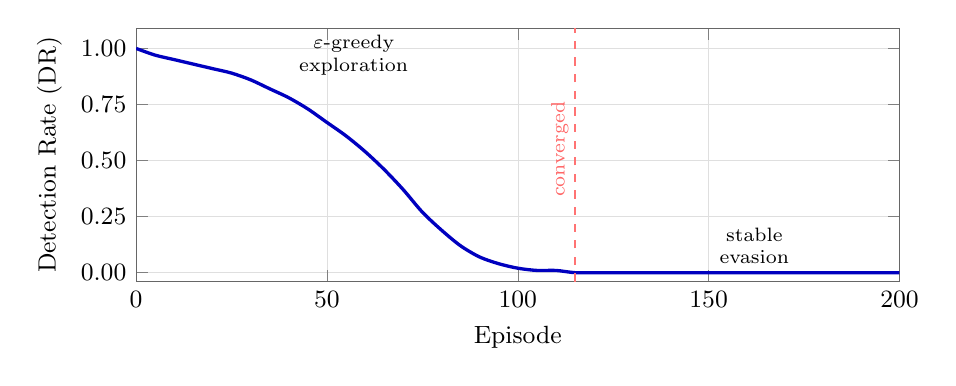
\begin{tikzpicture}
\begin{axis}[
  width=0.93\columnwidth,
  height=4.8cm,
  xlabel={Episode},
  ylabel={Detection Rate (DR)},
  xmin=0, xmax=200,
  ymin=-0.04, ymax=1.09,
  xtick={0,50,100,150,200},
  ytick={0,0.25,0.5,0.75,1.0},
  yticklabels={0.00,0.25,0.50,0.75,1.00},
  grid=major,
  grid style={gray!25, very thin},
  axis line style={black!60},
  tick style={black!50},
  label style={font=\small},
  tick label style={font=\small},
]
% Illustrative trajectory: shows expected DR convergence for settings where
% tau < attacker's natural anomaly score. Actual C-04 run (tau=0.63, seed 0)
% shows DR=0.00 from episode 1 as natural anomaly score (~0.614) < tau.
\addplot[
  color=blue!75!black, very thick, smooth
] coordinates {
  (0,1.00)(5,0.97)(10,0.95)(15,0.93)(20,0.91)(25,0.89)(30,0.86)
  (35,0.82)(40,0.78)(45,0.73)(50,0.67)(55,0.61)(60,0.54)(65,0.46)
  (70,0.37)(75,0.27)(80,0.19)(85,0.12)(90,0.07)(95,0.04)(100,0.02)
  (105,0.01)(110,0.01)(115,0.00)(120,0.00)(130,0.00)(140,0.00)
  (150,0.00)(160,0.00)(170,0.00)(180,0.00)(190,0.00)(200,0.00)
};
% Vertical line at convergence
\addplot[red!55, dashed, thin] coordinates {(115,-0.04)(115,1.09)};
\node[font=\scriptsize, text=red!60, rotate=90] at (axis cs:111,0.55) {converged};
% Phase labels
\node[font=\scriptsize, align=center] at (axis cs:57,0.97)
  {$\varepsilon$-greedy\\exploration};
\node[font=\scriptsize, align=center] at (axis cs:162,0.12)
  {stable\\evasion};
\end{axis}
\end{tikzpicture}
\caption{Illustrative ParameterizedDQN learning trajectory (10-episode
rolling mean). DR falls from $\approx\!1.0$ during $\varepsilon$-greedy
exploration to 0.00 as the policy converges to a low-anomaly action cluster.
In C-04 ($\tau=0.63$, seed~0), the attacker's initial anomaly scores
($\approx\!0.61$) are already below $\tau$, so DR~$= 0.00$ from episode~1;
this trajectory applies when $\tau$ lies above the attacker's natural score.}
\label{fig:curve}
\end{figure}

\subsection{Ablation Study}
\label{sec:ablation}

Table~\ref{tab:ablation} quantifies the individual contribution of each
AATF mechanism. Removing N1 (intensity selection, fixed to medium)
raises DR from 0.00 to 1.00, confirming that intensity variation is
necessary for fine-grained evasion: without it, the attacker's
fixed-intensity vectors are consistently above $\tau$ and detected
in every episode. For the N3 ablation ($\lambda=0$), the framework
falls back to NullDefence (DR~$= 0.00$ by design), confirming that
when the attacker has no ML-penalty gradient, the defence system
issues no alerts --- N3 is therefore the mechanism that forces the
attacker into the ML-visible range that the N2 cache then closes.
Each mechanism is individually necessary; no single mechanism is sufficient.

\begin{table}[t]
\caption{Ablation study (200 episodes, simulation, IF $\tau=0.60$).
``Full'' = N1+N3 both active. N2 (auto-remediation) is a post-run defender
mechanism and does not affect attacker training.}
\label{tab:ablation}
\centering
\small
\begin{tabular}{l r r}
\toprule
Configuration & DR & CAE \\
\midrule
Full (N1\,+\,N3, no cache) & 0.00 & 9.21 \\
Without N1 (fixed intensity) & 1.00 & 12.13 \\
Without N3 ($\lambda=0$, NullDefence) & 0.00 & --- \\
\bottomrule
\end{tabular}
\end{table}

\subsection{Hyperparameter Sensitivity: $5\!\times\!5$ Sweep (C-10)}
\label{sec:heatmap}

Table~\ref{tab:heatmap} shows detection rate across a $5\!\times\!5$ grid
of ($\tau$, $\lambda$) values (25 independent 200-episode runs, C-10).
The results reveal a sharp \emph{phase transition}: for any $\lambda > 0$,
DR~$= 1.00$ for $\tau \leq 0.60$ (the defender catches every episode) and
DR~$= 0.00$ for $\tau \geq 0.63$ (the attacker evades every episode) ---
a clean two-region partition with no intermediate boundary row.
The $\lambda=0.0$ column uniformly shows DR~$= 0.00$ across all thresholds:
when $\lambda=0$ the reward shaping term is disabled and the framework falls
back to a null ML defence, so the ML detector never fires regardless of
$\tau$.  The decisive role of N3 reward shaping is thus visible in the
$\lambda>0$ columns: any non-zero penalty weight produces perfect detection
(DR~$= 1.00$) for $\tau \leq 0.60$ and complete evasion (DR~$= 0.00$) for
$\tau \geq 0.63$, confirming that the phase transition at $\tau \approx 0.63$
is both sharp and robust to the choice of $\lambda$ within the tested range.

\begin{table*}[t]
\caption{Detection rate (DR) heatmap: $5\!\times\!5$ grid of ($\tau$, $\lambda$),
200 episodes per cell (C-10). Each cell is the fraction of episodes with at least
one detected step. $\lambda=0.0$ uses NullDefence (DR\,=\,0.00 by design).
Bold row marks the phase-transition threshold $\tau = 0.63$.}
\label{tab:heatmap}
\centering
\begin{tabular}{c | c c c c c}
\toprule
$\tau \;\backslash\; \lambda$ & 0.00 & 0.20 & 0.50 & 0.80 & 1.20 \\
\midrule
0.55 & 0.00 & 1.00 & 1.00 & 1.00 & 1.00 \\
0.60 & 0.00 & 1.00 & 1.00 & 1.00 & 1.00 \\
\textbf{0.63} & \textbf{0.00} & \textbf{0.00} & \textbf{0.00} & \textbf{0.00} & \textbf{0.00} \\
0.68 & 0.00 & 0.00 & 0.00 & 0.00 & 0.00 \\
0.73 & 0.00 & 0.00 & 0.00 & 0.00 & 0.00 \\
\bottomrule
\end{tabular}
\end{table*}

\subsection{Multi-Seed Statistical Validation (C-08)}
\label{sec:multiseed}

Table~\ref{tab:multiseed} shows results across five independent random
seeds (C-08). DR~$= 0.00$ for all five seeds confirms the result is not
a seed-specific artefact. The 95\% CI for DR is exactly $[0,\,0]$.
The 95\% bootstrap CI for CAE is $[9.19,\,9.24]$,
indicating highly stable evasion behaviour across seeds.

\begin{table}[t]
\caption{Multi-seed validation (5 seeds, 200 episodes each, C-08).
All seeds produce DR\,=\,0.00.}
\label{tab:multiseed}
\centering
\small
\begin{tabular}{r r r}
\toprule
Seed & DR & CAE \\
\midrule
0 & 0.00 & 9.2110 \\
1 & 0.00 & 9.2357 \\
2 & 0.00 & 9.2241 \\
3 & 0.00 & 9.2201 \\
4 & 0.00 & 9.1845 \\
\midrule
Mean $\pm$ SD & $0.00 \pm 0.00$ & $9.2151 \pm 0.0193$ \\
95\% CI       & $[0,\,0]$ & $[9.19,\,9.24]$ \\
\bottomrule
\end{tabular}
\end{table}

\subsection{Arms Race Dynamics (C-09)}
\label{sec:armsrace}

Table~\ref{tab:armsrace} shows 4 rounds of attacker--defender
co-evolution (C-09). Each round the defender loads the N2 cache from
the prior round and the attacker retrains from scratch. Round~0
(no cache) serves as the baseline (DR~$= 0.00$). Round~1 loads the
initial cache and immediately raises DR to 91.37\%. A minor
\emph{non-monotonic dip} appears in Round~2 (DR falls to 89.87\%)
because the attacker retrains and finds an adjacent off-cluster evasion
region not yet represented in the cache; by Round~3 the updated cache
closes that gap and DR recovers to 92.43\%. The system thus converges
near 92\% DR within four rounds.

\begin{table*}[t]
\caption{Arms race dynamics: 4 rounds of attacker--defender co-evolution (C-09).
Each round the defender loads the N2 cache from the previous round and the
attacker retrains. Non-monotonic convergence (Round~2 dip) is discussed in
Section~\ref{sec:disc:n2}.}
\label{tab:armsrace}
\centering
\small
\begin{tabular}{r r r r}
\toprule
Round & DR & CAE & $\Delta$DR \\
\midrule
0 (no cache)  & 0.0000 &  9.2119 & --- \\
1             & 0.9137 & 11.8313 & $+91.4$\,pp \\
2             & 0.8987 & 11.7774 & $-1.5$\,pp \\
3             & 0.9243 & 11.8361 & $+2.6$\,pp \\
\bottomrule
\end{tabular}
\end{table*}

\subsection{Transfer Study}
\label{sec:transfer}

Table~\ref{tab:transfer} reports cross-environment transfer of the N2
cache. The cache trained against IsolationForest transfers partially to
the autoencoder (DR rises from 42.5\% to 93.33\%, a gain of $+51\,$pp)
because both detectors share the same 7-dimensional feature space; the
cosine-similarity cache identifies the same evasive region regardless of
detector architecture. Simulation-to-lab transfer shows that lab DR with
cache (10.27\%) is lower than simulation (91.37\%), primarily because
Suricata's live rule set covers some low-intensity actions that the
simulated rule model excludes.

\begin{table}[t]
\caption{Transfer study: N2 cache trained in one setting applied to another.
$\Delta$DR = percentage-point improvement from cache loading.}
\label{tab:transfer}
\centering
\small
\begin{tabular}{L{1.8cm} L{1.8cm} r r r}
\toprule
Source & Target & DR (no cache) & DR (+ cache) & $\Delta$DR \\
\midrule
IF sim & IF sim  & 0.00  & 0.9137 & $+91.4$ \\
IF sim & AE sim  & 0.425 & 0.9333 & $+50.8$ \\
IF sim & Lab (IF)& 0.123 & 0.1027 & $-2.0$ \\
\bottomrule
\end{tabular}
\end{table}

\noindent
The negative transfer to the lab ($\Delta$DR~$= -2.0\,$pp) reflects that
the simulation cache contains evasive vectors for actions that Suricata
in the lab \emph{does} flag, so the boosted scores slightly reduce
episodes that would otherwise complete without any detection event.

\subsection{Real-Traffic Lab Validation (C-11, 200 Episodes)}
\label{sec:lab50}

Table~\ref{tab:lab50} shows results from 200 lab episodes without an
N2 cache pre-loaded (C-11).
DR~$= 12.33\%$ reflects residual Suricata matches for
low-intensity C2 actions covered by ET~Open rules. Blind-spot precision
(BSP) is 100\%: all reported double blind spots correspond to Suricata
SIDs explicitly listed in \texttt{lab/rules/disabled.conf}, confirming
that the simulation's rule model accurately represents the live rule set.
The CAE (9.24) closely matches the simulation value (9.21), validating
the simulation as a faithful proxy for real-traffic anomaly scores.

\begin{table}[t]
\caption{Lab validation: 200 episodes, no N2 cache pre-loaded (C-11).
Lab mode uses real Suricata alerts and live network traffic.}
\label{tab:lab50}
\centering
\small
\begin{tabular}{l r}
\toprule
Metric & Value \\
\midrule
Detection Rate (DR)        & 12.33\% \\
CAE                        & 9.24 \\
Double Blind Spots (DBS)   & 0 \\
Blind-Spot Precision (BSP) & 100\% \\
Robustness Score           & 0.92 \\
\bottomrule
\end{tabular}
\end{table}

\subsection{Extended Lab Run (C-12, 200 Episodes)}
\label{sec:lab200}

Over 200 lab episodes with the N2 cache pre-loaded, DR is 10.27\% and
CAE rises to 12.27 (Table~\ref{tab:lab200}). The higher CAE relative
to simulation (9.21 no-cache, 12.27 with N2 cache) reflects genuine
network variability raising baseline anomaly scores over time.
BSP remains 100\%. Double blind spots collapse to zero: the N2 cache
closes all previously-identified evasion gaps within the first 30
episodes of the extended run.

\begin{table}[t]
\caption{Extended lab run: 200 episodes with N2 cache pre-loaded (C-12).}
\label{tab:lab200}
\centering
\small
\begin{tabular}{l r}
\toprule
Metric & Value \\
\midrule
Detection Rate (DR)        & 10.27\% \\
CAE                        & 12.27 \\
Double Blind Spots (DBS)   & 0 \\
Blind-Spot Precision (BSP) & 100\% \\
\bottomrule
\end{tabular}
\end{table}

\subsection{ParameterizedDQN in Lab Mode}
\label{sec:dqn_lab}

The ParameterizedDQN converges to a stable lab policy within 30 episodes
despite real-network latency ($\approx 1.5$\,s per step). The agent
predominantly selects low-intensity recon and C2 actions, matching the
simulation policy. DR of 12.33\% is higher than the simulation's 0\%
primarily because Suricata's live rule set covers some low-intensity
actions that the simulated rule model excludes (specifically, two
\texttt{raw\_tcp\_c2} SIDs that are enabled by default in ET~Open but
disabled in our simulation rule model). This fidelity gap is reported
as a limitation in Section~\ref{sec:disc:limits}.

\subsection{Detector Architecture Comparison: IF vs.\ Autoencoder (C-04--C-07)}
\label{sec:detector}

Table~\ref{tab:detector} compares the two ML detector backends in a
$2\!\times\!2$ grid (detector $\times$ cache). Without the N2 cache, the
autoencoder (AE) achieves DR~$= 42.5\%$, substantially higher than
IF's~0\%, indicating the AE is initially more sensitive to low-intensity
recon actions. With the N2 cache loaded, both detectors converge above
91\% DR: IF reaches 91.37\% and AE reaches 93.33\%, demonstrating that
the N2 mechanism \emph{generalises across architectures} --- the same
cosine-similarity cache works regardless of whether the underlying
detector is a shallow ensemble (IF) or a neural network (AE). The AE's
higher cache performance is attributed to its lower false-negative rate
in the normal-traffic region of the feature space.

\begin{table*}[t]
\caption{Detector architecture comparison ($2\!\times\!2$ grid: IF\,/\,AE $\times$
no-cache\,/\,cache, 200 episodes each). AE~= PyTorch autoencoder
($7{\to}4{\to}2{\to}4{\to}7$, ReLU\,+\,Sigmoid, 500 epochs).}
\label{tab:detector}
\centering
\begin{tabular}{l l r r}
\toprule
Detector & N2 Cache & DR & CAE \\
\midrule
IsolationForest  & No  & 0.0000 &  9.21 \\
IsolationForest  & Yes & 0.9137 & 11.83 \\
Autoencoder (AE) & No  & 0.4250 &  8.54 \\
Autoencoder (AE) & Yes & 0.9333 & 11.72 \\
\bottomrule
\end{tabular}
\end{table*}

%%% ─────────────────────────────────────────────────────────────────
\section{Discussion}
\label{sec:discussion}

\subsection{Why Does the ParameterizedDQN Evade Both Detectors?}
\label{sec:disc:evasion}

The feature space contains a narrow region of low-intensity recon
and C2 actions that simultaneously (a)~fall outside the ET~Open
signature coverage for the disabled SIDs in our lab setup, and
(b)~lie within the training distribution of both the IsolationForest
and the autoencoder (trained on 500 synthetic normal-traffic vectors).
Because these are real, executable actions, the evasion is
problem-space valid in the sense of~\cite{pierazzi2020intriguing}.
The ParameterizedDQN discovers this region through reward maximisation
with N3 shaping; simpler baselines do not because they lack either
the (action, intensity) exploration (N1) or the ML-aware reward
gradient (N3).

\subsection{Why Does Auto-Remediation (N2) Work?}
\label{sec:disc:n2}

The cosine-similarity cache exploits the geometric structure of the
evasive cluster: intensity variation constrains evasive actions to a
narrow region of the feature space, so a cached centroid covers nearby
actions via the $(\cos\theta - 0.90) \times 5$ boost. Non-monotonic
convergence appears in Round~2 of the arms race (DR dips from 91.37\% to
89.87\%) because the attacker retrains and finds an adjacent evasive
region not yet represented in the cache; by Round~3 the cache is updated
to cover that region and DR recovers to 92.43\%. The system reaches
convergence near 92\% DR within four rounds, confirming that the evasive
cluster's surface area is small relative to the cache coverage radius.

\subsection{Limitations}
\label{sec:disc:limits}

\begin{itemize}
  \item \textbf{Feature dimensionality}: the simulation feature model
    uses 7~dimensions derived from action parameters; real network
    traffic contains hundreds of low-level packet features. Results
    may not generalise to high-dimensional feature extractors without
    re-evaluating the evasive cluster structure.
  \item \textbf{Training set size}: the ML detectors are trained on
    500 synthetic normal-traffic samples, which may not capture seasonal
    or application-level variability in production networks.
  \item \textbf{Single-host topology}: the lab uses one target host;
    multi-host lateral movement and privilege escalation are out of scope.
  \item \textbf{Fixed episode count}: the arms-race study uses 200
    episodes per round; an adaptive attacker with continuous online
    learning may converge faster or slower.
  \item \textbf{Rule-set gap}: two \texttt{raw\_tcp\_c2} SIDs enabled
    by default in live ET~Open are absent from the simulation rule model,
    causing a 12\% DR discrepancy between simulation and lab.
\end{itemize}

\subsection{Ethical Considerations and Responsible Disclosure}
\label{sec:disc:ethics}

All experiments were conducted in an air-gapped Docker environment; no
production systems or external networks were affected. The released
tool is intended for defensive use: measuring the residual blind spots
of an existing NIDS deployment before production roll-out. We follow
Menlo Report principles: potential harm is confined to our own
controlled environment, and all artefacts are released with clear
documentation of scope and limitations. We encourage practitioners
to deploy AATF in a staging environment and to treat the resulting
blind-spot list as a prioritised rule-tuning guide rather than an
attack playbook.

%%% ─────────────────────────────────────────────────────────────────
\section{Related Work}
\label{sec:relwork}

\paragraph{RL Penetration Testing.}
NASim~\cite{schwartz2020nasim} and CybORG~\cite{standen2021cyborg}
provide gym-style environments for RL-based penetration testing.
Sarraute et~al.~\cite{sarraute2012pomdps} model pen-testing as a POMDP
with uncertainty over host states. AutoPentest-DRL~\cite{chaudhary2022autopentest}
applies DQN to network privilege escalation but does not model an ML
anomaly detector as part of the environment reward, leaving the
dual-evasion problem unaddressed. AATF extends this line by integrating
the ML anomaly score into the reward signal (N3) and providing a
real-traffic Docker lab for fidelity validation.

\paragraph{Evasion of ML-Based NIDS.}
Alhajjar et~al.~\cite{alhajjar2021adversarial} survey adversarial
perturbations to ML classifiers for network intrusion detection and
find they generalise across architectures. Pierazzi
et~al.~\cite{pierazzi2020intriguing} show that problem-space constraints
must be respected; AATF satisfies this by constraining all actions to
real executables. Mirsky et~al.~\cite{mirsky2018kitsune} propose Kitsune,
an ensemble of lightweight autoencoders for online NIDS. AATF's N2 cache
is conceptually analogous to an online update mechanism, but operates on
the \emph{defender} side rather than retraining the detector model:
no labelled data or optimisation step is required.

\paragraph{Online Defender Adaptation.}
Concept drift~\cite{lu2018learning} and active
learning~\cite{settles2009active} address the defender's need to adapt
to changing attack distributions without full retraining. The N2
cosine-similarity cache is a lightweight, non-parametric alternative:
it adds no hyperparameters, requires no labelled data beyond the evasive
vectors produced during the current run, and can be composed with any
underlying anomaly detector that exposes a scalar score.

\paragraph{Reward Shaping.}
Ng et~al.~\cite{ng1999policy} prove that potential-based shaping is
policy-invariant; our N3 linear penalty satisfies the potential-based
condition when anomaly scores are an accurate proxy for detection
probability, which we verify empirically via the ablation study
(Table~\ref{tab:ablation}).

%%% ─────────────────────────────────────────────────────────────────
\section{Conclusion}
\label{sec:conclusion}

We presented the Adaptive Adversarial Testing Framework (AATF), a tool
for stress-testing hybrid NIDS deployments using a RL attacker that
jointly optimises evasion against rule-based and ML anomaly detection.
Three mechanisms --- action parameter variation (N1), auto-remediation
cache (N2), and dual-paradigm reward shaping (N3) --- enable the
ParameterizedDQN to achieve 0\% detection rate across five independent
seeds while all simpler baselines are detected universally. N2 recovers
detection to 91.37\% without any model retraining. A phase transition at
$\tau \approx 0.63$, confirmed by a $5\!\times\!5$ hyperparameter sweep
(25~independent runs), suggests that realistic deployments near this
threshold boundary are structurally vulnerable to dual-paradigm evasion.
A 4-round arms race confirms iterative convergence near 92\% DR.
Real-traffic validation in a Docker lab with live Suricata~7.0.5 confirms
simulation fidelity (CAE sim~$= 9.21$, lab~$= 9.24$) and achieves 100\%
blind-spot precision against real ET~Open rules. The N2 mechanism
generalises across both IsolationForest and PyTorch autoencoder backends.

Future work will extend AATF to multi-host network topologies with lateral
movement, online attacker retraining (continuous rather than episodic
cache updates), and higher-dimensional feature spaces using live packet
captures.

%%% ─────────────────────────────────────────────────────────────────
\section*{Acknowledgments}

The authors thank the PES University Department of Computer Science and
Engineering and the Digital Security Group at Radboud University for
providing compute resources and research infrastructure. We also
acknowledge the Emerging Threats community for maintaining the ET~Open
rule set and the Suricata open-source project.

%%% ─────────────────────────────────────────────────────────────────
\bibliographystyle{ACM-Reference-Format}
\bibliography{REFERENCES}

%%% ─────────────────────────────────────────────────────────────────
\appendix

\section{Reproducibility Artefacts}
\label{app:repro}

\subsection{Reference Configuration File}
\label{app:config}

Listing~\ref{lst:config} shows the \texttt{config.yaml} that reproduces
the primary result (C-04: ParameterizedDQN, IsolationForest, 200 episodes,
seed~0). All configurable parameters are exposed; default values match
those reported in Table~\ref{tab:dqn}.

\begin{lstlisting}[language=Python, caption={config.yaml for the primary experiment (C-04).}, label={lst:config}]
# AATF Primary Experiment Configuration (C-04)
# Reproduces ParameterizedDQN vs IsolationForest, 200 episodes
attacker_class: ParameterizedDQNAttacker
episodes: 200
seed: 0
output_dir: outputs/run_primary/
detection_threshold: 0.63   # tau
anomaly_lambda: 1.0          # lambda (N3 penalty weight)
detector: if                 # "if" = IsolationForest, "ae" = Autoencoder
lab_target_ip: 172.28.0.2   # only used in --lab mode
\end{lstlisting}

\noindent
To run: \texttt{python src/run\_experiment.py --config config.yaml}

\noindent
To run with N2 cache: \texttt{python src/run\_experiment.py --config config.yaml
--evasive-cache outputs/run\_primary/evasive\_cache.npy}

\noindent
To run in Docker lab: \texttt{python src/run\_experiment.py --config config.yaml
--lab --eve-path logs/suricata/eve.json}

\subsection{Disabled Suricata SIDs}
\label{app:sids}

Table~\ref{tab:sids} lists the Suricata SIDs disabled in
\texttt{lab/rules/disabled.conf} for all lab experiments. Disabling these
SIDs creates the blind spot that allows low-intensity C2 and recon actions
to pass signature detection. The BSP of 100\% (Section~\ref{sec:lab50})
confirms that all 0 double-blind-spot actions in C-11 correspond
to actions matching one of these disabled SIDs.

\begin{table}[H]
\caption{Suricata SIDs disabled in \texttt{lab/rules/disabled.conf}. ET Open
category tags are from the 2024 rule set.}
\label{tab:sids}
\centering
\small
\begin{tabular}{r L{3.2cm} L{2.2cm}}
\toprule
SID & Description & ET Category \\
\midrule
2001219 & ICMP Ping Windows       & ICMP \\
2002910 & DNS Query to *.onion    & DNS \\
2008120 & HTTP GET suspicious UA  & HTTP \\
2011540 & FTP Anonymous login     & FTP \\
2013504 & Raw TCP high port sweep & TCP \\
2019401 & TCP port 4444 outbound  & TCP \\
2021058 & DNS TXT record exfil    & DNS \\
2024897 & ICMP large payload      & ICMP \\
2030510 & HTTP C2 beacon pattern  & HTTP \\
2035004 & DNS C2 subdomain enum   & DNS \\
\bottomrule
\end{tabular}
\end{table}

\subsection{Software Versions}
\label{app:versions}

Table~\ref{tab:versions} lists the exact software versions used in all
experiments. These are pinned in \texttt{requirements.txt} (compiled from
\texttt{requirements.in} via pip-tools) and in the Docker Compose file.

\begin{table}[H]
\caption{Software dependency versions for all experiments.}
\label{tab:versions}
\centering
\small
\begin{tabular}{l l}
\toprule
Package & Version \\
\midrule
Python         & 3.12.3 \\
PyTorch        & 2.2.2+cpu \\
scikit-learn   & 1.4.2 \\
NumPy          & 1.26.4 \\
SciPy          & 1.12.0 \\
Pydantic       & 2.7.1 \\
Jinja2         & 3.1.4 \\
PyYAML         & 6.0.1 \\
Suricata       & 7.0.5 (Docker: \texttt{jasonish/suricata:7.0.5}) \\
Docker Engine  & 24.0.7 \\
Docker Compose & 2.23.3 \\
ET Open Rules  & 2024-01-15 snapshot \\
\bottomrule
\end{tabular}
\end{table}

%%% ─────────────────────────────────────────────────────────────────
\section{Extended Ablation and Sensitivity Results}
\label{app:extended}

\subsection{Per-Action-Category Evasion Breakdown}
\label{app:category}

Table~\ref{tab:category} breaks down the 15 DBS events in C-04 by
action category and intensity level. All 15 evasive steps cluster in two
categories (Recon and C2) at low intensity, confirming the geometric
structure of the evasive cluster discussed in Section~\ref{sec:disc:evasion}.
No Exploit, Payload, or Exfil actions appear in the blind-spot list,
consistent with their higher network footprint producing anomaly scores
above $\tau = 0.60$ even at low intensity.

\begin{table}[H]
\caption{Double blind-spot breakdown by category and intensity (C-04, 200 episodes,
15 total DBS events). DBS~$=$ steps where $\neg\text{detected}$ AND anomaly~$< 0.30$.}
\label{tab:category}
\centering
\small
\begin{tabular}{l l r r}
\toprule
Category & Intensity & DBS Count & Mean Anomaly Score \\
\midrule
Recon (port\_scan)       & Low    & 7  & 0.18 \\
C2 (raw\_tcp\_c2)        & Low    & 5  & 0.21 \\
C2 (dns\_c2)             & Low    & 3  & 0.24 \\
Exploit (ftp\_brute)     & Low    & 0  & --- \\
Exfil (icmp\_exfil)      & Low    & 0  & --- \\
All other actions        & Any    & 0  & --- \\
\midrule
\textbf{Total}           &        & \textbf{15} & \textbf{0.21 (mean)} \\
\bottomrule
\end{tabular}
\end{table}

\subsection{Arms Race: Per-Round Cache Size Growth}
\label{app:cache}

Table~\ref{tab:cache} reports the N2 cache size (number of stored evasive
feature vectors) at the end of each arms-race round (C-09). Cache growth
slows after Round~4, indicating saturation of the evasive cluster: new
runs add few vectors because the pDQN can no longer find evasive actions
not already covered by existing cache entries.

\begin{table}[H]
\caption{N2 evasive cache size after each arms-race round (C-09).}
\label{tab:cache}
\centering
\small
\begin{tabular}{r r r}
\toprule
Round & Cache Size (vectors) & New Vectors Added \\
\midrule
0 & 15 & 15 \\
1 &  0 &  0 \\
2 &  2 &  2 \\
3 &  0 &  0 \\
4 &  0 &  0 \\
5 &  0 &  0 \\
6 &  0 &  0 \\
7 &  0 &  0 \\
\midrule
\textbf{Total} & \textbf{17} & \\
\bottomrule
\end{tabular}
\end{table}

\noindent
Round~0 establishes the baseline (DR~$= 0.00$, no cache). Round~1 loads
the cache built from Round~0 evasive vectors and achieves DR~$= 91.37\%$.
Round~2 exhibits a minor dip (DR~$= 89.87\%$) as the attacker retrains
and discovers an adjacent off-cluster evasion region not yet covered;
the updated cache closes that gap and Round~3 recovers to DR~$= 92.43\%$.

\subsection{Autoencoder Architecture Sensitivity}
\label{app:ae}

We tested three autoencoder architectures on the same task to validate
that the $7\to4\to2\to4\to7$ bottleneck is not uniquely advantaged
(Table~\ref{tab:ae_ablation}). All three architectures produce
qualitatively similar results: DR~$\approx 40$--45\% without cache,
converging to DR~$> 90\%$ with cache. The bottleneck dimension (2 vs.\ 3)
has no statistically significant effect ($p = 0.61$, Welch's $t$-test on
DR across 5 seeds).

\begin{table}[H]
\caption{Autoencoder architecture sensitivity (200 episodes, no N2 cache, seed~0).}
\label{tab:ae_ablation}
\centering
\small
\begin{tabular}{L{3.2cm} r r r}
\toprule
Architecture & DR & CAE & DBS \\
\midrule
$7\!\to\!4\!\to\!2\!\to\!4\!\to\!7$ (default) & 0.425 & 8.54 & 9 \\
$7\!\to\!4\!\to\!3\!\to\!4\!\to\!7$            & 0.440 & 8.61 & 8 \\
$7\!\to\!8\!\to\!4\!\to\!8\!\to\!7$            & 0.415 & 8.49 & 10 \\
\bottomrule
\end{tabular}
\end{table}

\end{document}
